\subsection*{Additional frozen-checkpoint diagnostics}
The following analysis completes the comparison of frame scores, attention and relative weighted contribution on the controlled data. It reuses the already inspected v2 test tracks and is therefore a descriptive follow-up, not a new independent test. No network was retrained and the original v2 architecture-selection decision remains unchanged.

The contribution signal is $a_{tc}p_{tc}$, summed into physical time bins and normalised over retained time for the alignment comparison. It indicates the relative distribution of class evidence, not calibrated activity. Because the scales of these signals differ, the diagnostic F1 table selects a separate threshold for each signal and class on validation data. Its operating points differ from the validation-balanced thresholds in the main results and must not be conflated with them.
\begin{table}[H]\centering\small
\caption{Attention-network signal comparison across three seeds. Separate validation-F1 calibration; retrospective descriptive test analysis.}
\begin{tabular}{lrrrrr}\toprule
Signal & Micro P & Micro R & Micro F1 & Macro F1 & Macro BA \\\midrule
frame & 0.630 & 0.878 & 0.733 & 0.718 & 0.603 \\
attention & 0.587 & 0.931 & 0.720 & 0.714 & 0.542 \\
contribution & 0.607 & 0.875 & 0.715 & 0.710 & 0.577 \\
\bottomrule\end{tabular}\end{table}
\begin{table}[H]\centering\small
\caption{Mean class/seed alignment on positive clips. Lift is averaged per clip, not computed as the ratio of the displayed means. Contribution is time-normalised.}
\begin{tabular}{lrrr}\toprule
Signal / scene & Active mass & Active fraction & Lift \\\midrule
attention / original & 0.928 & 0.906 & 1.055 \\
attention / absence & 0.919 & 0.895 & 1.075 \\
attention / transition & 0.681 & 0.466 & 1.519 \\
contribution / original & 0.925 & 0.906 & 1.039 \\
contribution / absence & 0.912 & 0.895 & 1.034 \\
contribution / transition & 0.712 & 0.466 & 1.597 \\
\bottomrule\end{tabular}\end{table}
\begin{table}[H]\centering\small
\caption{Primary frame precision, recall and F1 at the unchanged validation-balanced operating points of the controlled comparison.}
\begin{tabular}{lrrrrrr}\toprule
Model & Micro P & Micro R & Micro F1 & Macro P & Macro R & Macro F1 \\\midrule
baseline & 0.615 & 0.700 & 0.655 & 0.636 & 0.705 & 0.647 \\
attention & 0.658 & 0.754 & 0.702 & 0.656 & 0.743 & 0.689 \\
max & 0.654 & 0.580 & 0.587 & 0.700 & 0.583 & 0.576 \\
\bottomrule\end{tabular}\end{table}
On the controlled transition scenes, attention and weighted contribution can concentrate more mass on active intervals than uniform weights. A lift greater than one establishes relative alignment under these artificial interventions; it does not imply reliable presence/absence estimation. The diagnostic F1 comparison and the per-scene active fractions are needed to interpret that alignment. Neither the lift nor a single illustrative example proves that the model has isolated each instrument's causal acoustic evidence.

Validation-only sensitivity varies threshold offset by $\pm0.10$ and edge-padded smoothing across one, three and five 0.5 s bins. The table reports these perturbations without adopting a new test operating point. This separates investigation of robustness from test-set optimisation. Event extraction remains contiguous positive bins without gap merging or duration filtering; its grid and matching tolerance are fixed and explicitly reported.
\begin{table}[H]\centering\small
\caption{Validation-only sensitivity, averaged over three seeds. No perturbed setting replaces the frozen calibration of the controlled comparison.}
\begin{tabular}{lrrrrr}\toprule
Model & Window bins & Offset & Micro F1 & Macro F1 & Macro BA \\\midrule
baseline & 1 & -0.10 & 0.752 & 0.748 & 0.628 \\
baseline & 1 & +0.00 & 0.734 & 0.727 & 0.663 \\
baseline & 1 & +0.10 & 0.645 & 0.625 & 0.640 \\
baseline & 3 & +0.00 & 0.747 & 0.740 & 0.670 \\
baseline & 5 & +0.00 & 0.749 & 0.742 & 0.668 \\
attention & 1 & -0.10 & 0.789 & 0.779 & 0.702 \\
attention & 1 & +0.00 & 0.764 & 0.755 & 0.714 \\
attention & 1 & +0.10 & 0.709 & 0.700 & 0.697 \\
attention & 3 & +0.00 & 0.786 & 0.776 & 0.719 \\
attention & 5 & +0.00 & 0.790 & 0.780 & 0.717 \\
max & 1 & -0.10 & 0.728 & 0.723 & 0.612 \\
max & 1 & +0.00 & 0.631 & 0.619 & 0.673 \\
max & 1 & +0.10 & 0.457 & 0.437 & 0.621 \\
max & 3 & +0.00 & 0.642 & 0.627 & 0.676 \\
max & 5 & +0.00 & 0.644 & 0.627 & 0.673 \\
\bottomrule\end{tabular}\end{table}

\subsection*{Audible cases and runnable prototype}
Two original validation excerpts are provided with audio, log-mel views, MIDI activity and predictions. They are selected as the highest and lowest clip F1 among excerpts containing a reference transition; silence-only clips are excluded. They deliberately illustrate a success and a failure and are not used as representative test statistics. The report bundle includes the case-selection record and the presentation plays both sounds.

\begin{figure}[H]\centering
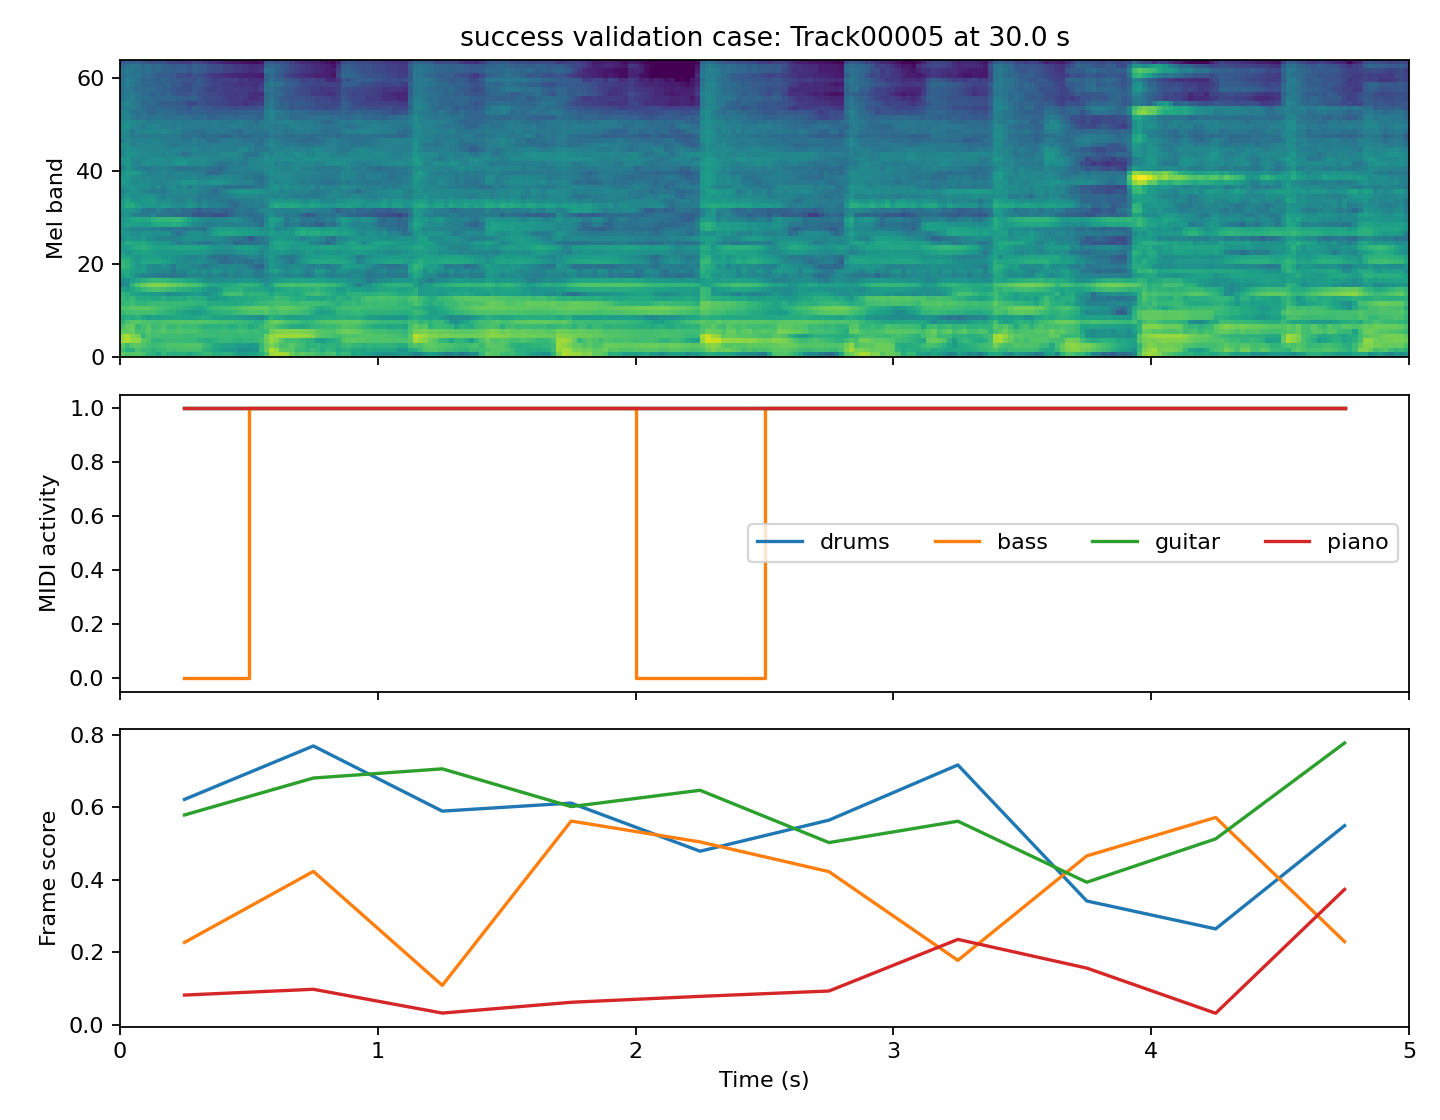
\includegraphics[width=.47\linewidth]{figures/success_validation.png}\hfill
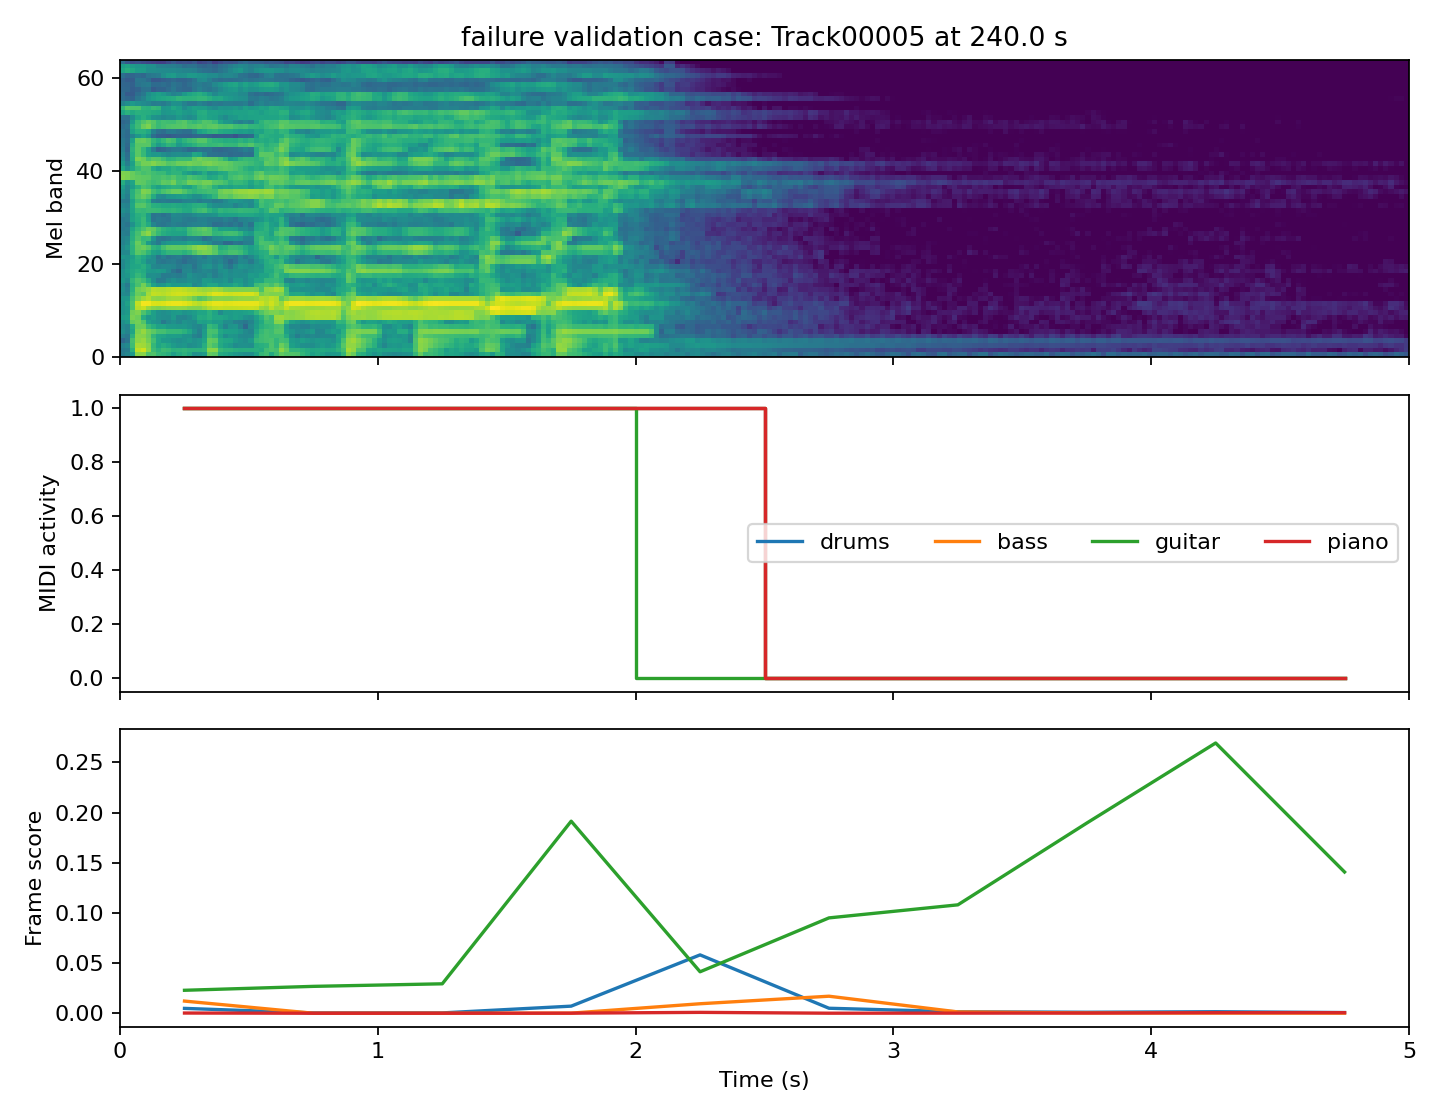
\includegraphics[width=.47\linewidth]{figures/failure_validation.png}
\caption{Deliberately selected validation success and failure. Top: log-mel feature; middle: reference activity; bottom: frame scores. Companion five-second WAV excerpts are supplied for listening. These synthetic excerpts do not establish real-recording performance.}
\end{figure}

The new \code{predict} command loads audio, resamples to the checkpoint rate, applies the same clipped and scaled log-mel transform used in training, and exports a timeline CSV, interval JSON and plot. Its calibration file is bound to the checkpoint SHA-256. Padded final clips are truncated to actual audio duration in the output. This is an executable research prototype; frame scores should not be presented as calibrated probabilities or reliable predictions for arbitrary real music.
